\chapter{Optical Properties of Semiconductor}
\section{Maxwell Equations and Vector Potential}
The properties of electromagnetic fields in a medium are described by the four Maxwell equations. Apart from the electric field \( \mathbf{F} \), magnetic field \( \mathbf{B} \), and velocity of light, the effects of the material are represented by the dielectric constant \( \varepsilon \), permeability \( \mu \) (assumed \( \mu = \mu_0 \)), and electrical conductivity.
We start with the four Maxwell equations:
\begin{equation}
	\nabla \times \mathbf{F} + \frac{\partial \mathbf{B}}{\partial t} = 0, \quad
	\nabla \times \mathbf{H} - \frac{\partial \mathbf{D}}{\partial t} = \mathbf{J}, \quad
	\nabla \cdot \mathbf{D} = \rho, \quad
	\nabla \cdot \mathbf{B} = 0
\end{equation}
Here, \( \mathbf{D} = \varepsilon \mathbf{F} \), \( \mathbf{B} = \mu \mathbf{H} \), and \( \mathbf{J} \), \( \rho \) are current and charge densities, respectively.
In electron-photon interactions, it is convenient to use the scalar and vector potentials \( \phi \) and \( \mathbf{A} \), defined by:
\begin{equation}
	\mathbf{F} = -\frac{\partial \mathbf{A}}{\partial t} - \nabla \phi, \quad
	\mathbf{B} = \nabla \times \mathbf{A}
\end{equation}
These definitions automatically satisfy the first and fourth Maxwell equations. The potentials \( \phi \) and \( \mathbf{A} \) are not unique, and can be transformed using the gauge transformation:
\begin{equation}
	\mathbf{A}' = \mathbf{A} + \nabla \chi, \quad \phi' = \phi - \frac{\partial \chi}{\partial t}
\end{equation}
These transformations do not affect the physical fields \( \mathbf{F} \) and \( \mathbf{B} \).\\
Rewriting the second and third Maxwell equations in terms of \( \phi \) and \( \mathbf{A} \), we get:
\begin{equation}
	\frac{1}{\mu_0} \nabla \times (\nabla \times \mathbf{A}) + \varepsilon \frac{\partial^2 \mathbf{A}}{\partial t^2} + \varepsilon \nabla \left( \frac{\partial \phi}{\partial t} \right) = \mathbf{J}
\end{equation}
\begin{equation}
	\frac{\partial}{\partial t}(\nabla \cdot \mathbf{A}) + \nabla^2 \phi = -\frac{\rho}{\varepsilon}
\end{equation}
Using the identity:
\begin{equation}
	\nabla \times (\nabla \times \mathbf{A}) = \nabla (\nabla \cdot \mathbf{A}) - \nabla^2 \mathbf{A}
\end{equation}
We obtain:
\begin{equation}
	-\nabla^2 \mathbf{A} + \varepsilon \mu_0 \frac{\partial^2 \mathbf{A}}{\partial t^2} + \nabla \left( \nabla \cdot \mathbf{A} + \varepsilon \frac{\partial \phi}{\partial t} \right) = \mu_0 \mathbf{J}
\end{equation}
We now impose the Lorentz gauge condition:
\begin{equation}
	\nabla \cdot \mathbf{A} + \varepsilon \frac{\partial \phi}{\partial t} = 0
\end{equation}
This simplifies the Maxwell equations to:
\begin{equation}
	\nabla^2 \mathbf{A} - \varepsilon \mu_0 \frac{\partial^2 \mathbf{A}}{\partial t^2} = -\mu_0 \mathbf{J}, \quad
	\nabla^2 \phi - \varepsilon \mu_0 \frac{\partial^2 \phi}{\partial t^2} = -\frac{\rho}{\varepsilon}
\end{equation}
This form is especially useful for generalization to relativistic electrodynamics. In the **Coulomb (radiation) gauge**, where \( \mathbf{J} = 0 \) and \( \rho = 0 \), we may set \( \phi = 0 \) and \( \nabla \cdot \mathbf{A} = 0 \). The vector potential becomes a solution of the wave equation, typically:
\begin{equation}
	\mathbf{A}(\mathbf{r}, t) = \mathbf{A}_0 \left[ e^{i(\mathbf{k} \cdot \mathbf{r} - \omega t)} + \text{c.c.} \right]
\end{equation}
Where the wavevector \( \mathbf{k} \) and angular frequency \( \omega \) satisfy:
\begin{equation}
	|\mathbf{k}|^2 = \varepsilon \mu_0 \omega^2
\end{equation}
The corresponding electric and magnetic fields are:
\begin{equation}
	\mathbf{F} = -\frac{\partial \mathbf{A}}{\partial t} = 2\omega \mathbf{A}_0 \sin(\mathbf{k} \cdot \mathbf{r} - \omega t)
\end{equation}
\begin{equation}
	\mathbf{B} = \nabla \times \mathbf{A} = - 2\mathbf{k} \times \mathbf{A}_0 \sin(\mathbf{k} \cdot \mathbf{r} - \omega t)
\end{equation}
The Poynting vector representing the optical power is:
\begin{align}
	\mathbf{S} & = (\mathbf{F} \times \mathbf{H})                                                                       \\
	           & = \frac{4 v k^2}{\mu_0} \left| A_0 \right|^2 \sin^2(\mathbf{k} \cdot \mathbf{r} - \omega t) \, \hat{k}
\end{align}
The average power carried by the electromagnetic wave in the medium, where \( v = \frac{c}{\sqrt{\tilde{\epsilon}}} \) is the speed of light in the material and \( \hat{k} \) is the propagation direction unit vector, can be expressed as:
\begin{equation}
	\langle \mathbf{S} \rangle_{\text{time}} = \hat{k} \, \frac{2 v k^2 |\mathbf{A}_0|^2}{\mu_0}
\end{equation}
By rewriting the wave vector magnitude \( |\mathbf{k}| \) in terms of the angular frequency and the wave velocity, i.e.,
\begin{equation}
	|\mathbf{k}| = \frac{\omega}{v}
\end{equation}
we can substitute into the expression for the time-averaged Poynting vector to obtain:
\begin{equation}
	\langle \mathbf{S} \rangle_{\text{time}} = 2 v \epsilon \mu_0 \omega^2 |\mathbf{A}_0|^2 \hat{k}
\end{equation}
The energy stored per unit volume in the electromagnetic field can be related to the Poynting vector and the wave velocity as
\begin{equation}
	\left| \frac{S}{v} \right| = \frac{2 \epsilon \omega^2 |\mathbf{A}_0|^2}{c^2}
\end{equation}
Assuming a photon population of \( n_{\text{ph}} \), the energy density in a volume \( V \) becomes
\begin{equation}
	\frac{n_{\text{ph}} \hbar \omega}{V}
\end{equation}
Equating the two energy densities, we can isolate the amplitude of the vector potential:
\begin{equation}
	|\mathbf{A}_0|^2 = \frac{n_{\text{ph}} \hbar}{2 \epsilon \omega V}
\end{equation}
With these foundational relations established, we now consider wave propagation in a medium. By substituting \( \mathbf{J} = \sigma \mathbf{F} \) into Maxwell's equations and eliminating the magnetic field, we obtain the wave equation for the electric field:
\begin{equation}
	\nabla^2 \mathbf{F} = \epsilon \mu_0 \frac{\partial^2 \mathbf{F}}{\partial t^2} + \sigma \mu_0 \frac{\partial \mathbf{F}}{\partial t}
\end{equation}
This equation describes a damped wave. A general solution takes the form
\begin{equation}
	\mathbf{F} = \mathbf{F}_0 \exp \{ i(\mathbf{k} \cdot \mathbf{r} - \omega t) \}
\end{equation}
Substituting this into the wave equation yields the relation for the wavevector magnitude:
\begin{equation}
	-k^2 = -\epsilon \mu_0 \omega^2 - \sigma \mu_0 i \omega
\end{equation}
Or more compactly,
\begin{equation}
	k = \frac{\omega}{c} \left( \tilde{\epsilon} + \frac{\sigma \mu_0 i}{\omega} \right)^{1/2}
\end{equation}
Here, \( \tilde{\epsilon} \) represents the relative dielectric constant. In vacuum, where \( \sigma = 0 \) and \( \tilde{\epsilon} = 1 \), the wavevector simplifies to
\begin{equation}
	k = \frac{\omega}{c}
\end{equation}
Within a material, the propagation speed is affected by a complex refractive index \( n_r \), defined by
\begin{equation}
	n_r = \left( \tilde{\epsilon} + \frac{\sigma \mu_0 i}{\omega} \right)^{1/2}
\end{equation}
We can express \( n_r \) in terms of its real and imaginary parts as
\begin{equation}
	n_r = n_r' + i n_r''
\end{equation}
Substituting this into the expression for \( k \), we obtain
\begin{equation}
	k = \frac{n_r' \omega}{c} + i \frac{n_r'' \omega}{c}
\end{equation}
The electric field wave for propagation in the \( +z \) direction can be written as

\begin{equation}
	\mathbf{F} = \mathbf{F}_0 \exp\left\{ i\omega \left( \frac{n_r' z}{c} - t \right) \right\} \exp\left( \frac{-n_r'' \omega z}{c} \right)
\end{equation}
Here, the phase velocity is reduced by a factor \( n_r' \), making it \( c / n_r' \), and the wave amplitude decays exponentially as \( \exp(-2\pi n_r'' / n_r') \) per wavelength. This decay in amplitude is a result of absorption of the electromagnetic energy.\\
The absorption coefficient \( \alpha \), which characterizes the intensity loss, is given by
\begin{equation}
	\alpha = \frac{2 n_r'' \omega}{c}
\end{equation}
In the special case where there is no absorption, the real part of the refractive index \( n_r' \) equals the total refractive index \( n_r \), and \( n_r'' = 0 \).\\
The absorption coefficient is measurable and provides direct information about the imaginary component \( n_r'' \) of the refractive index.\\
The interaction of the medium with the electromagnetic field is fully described by a complex dielectric constant or equivalently a complex refractive index. The real and imaginary parts of the dielectric constant \( \tilde{\epsilon} \) are related to the refractive index components as follows:
\begin{equation}
	\tilde{\epsilon}_1 = n_r'^2 - n_r''^2, \qquad
	\tilde{\epsilon}_2 = 2 n_r' n_r''
\end{equation}
These expressions relate the real (\( \tilde{\epsilon}_1 \)) and imaginary (\( \tilde{\epsilon}_2 \)) parts of the relative permittivity to the components of the complex refractive index.\\
A very significant relationship exists between the real and imaginary parts of the refractive index based on causality—this is known as the Kramers–Kronig relation. It connects the frequency-dependent refractive index to the absorption coefficient via
\begin{equation}
	n(\omega_0) - 1 = \frac{c}{\pi} \mathcal{P} \int_0^\infty \frac{\alpha(\omega)}{\omega^2 - \omega_0^2} \, d\omega
\end{equation}
This formulation is powerful as it enables the calculation of the refractive index if the absorption coefficient is known. In cases where the absorption spectrum varies under external influences (e.g., electric fields), changes in the refractive index can be predicted accordingly.


\section{Electrons in Electromagnetic Field}
Electrons, possessing a negative charge, interact with electric and magnetic fields originating from electromagnetic radiation. The electric field exerts a force equal to the product of the charge and the field itself, whereas the magnetic field contributes through the Lorentz force, which involves the cross product between the electron's velocity and the magnetic field.\\
This interaction energy defines the interaction Hamiltonian, which plays a central role in electron scattering processes. The total Hamiltonian for a charge \( e \) in the presence of an electromagnetic field is
\begin{equation}
	H = \frac{1}{2m_0} (\mathbf{p} - e \mathbf{A})^2 + e \phi + V(\mathbf{r})
\end{equation}
Expanding the square and rearranging terms:
\begin{equation}
	H = \frac{\mathbf{p}^2}{2m_0} - \frac{e}{2m_0} (\mathbf{p} \cdot \mathbf{A} + \mathbf{A} \cdot \mathbf{p}) + \frac{e^2}{2m_0} \mathbf{A}^2 + e \phi + V(\mathbf{r})
\end{equation}
In this expression, \( \mathbf{A} \) denotes the vector potential and \( V(\mathbf{r}) \) represents any potential due to the crystal lattice.\\
Within the framework of quantum mechanics, the momentum operator \( \mathbf{p} \) is defined differentially. Therefore, the operator form of \( \mathbf{p} \cdot \mathbf{A} \) becomes
\begin{equation}
	\frac{e}{2m_0} \mathbf{p} \cdot \mathbf{A} = \frac{e}{2m_0} \mathbf{A} \cdot \mathbf{p} - \frac{i e \hbar}{2m_0} \nabla \cdot \mathbf{A}
\end{equation}
Substituting this result into the Hamiltonian yields
\begin{equation}
	H = \frac{\mathbf{p}^2}{2m_0} - \frac{e}{m_0} \mathbf{A} \cdot \mathbf{p} + \frac{i e \hbar}{2m_0} \nabla \cdot \mathbf{A} + \frac{e^2}{2m_0} \mathbf{A}^2 + e \phi + V(\mathbf{r})
\end{equation}
To analyze the influence of electromagnetic radiation on an electron, we apply perturbation theory. In the quantum mechanical description of radiation, the electromagnetic field is represented using creation and annihilation operators, akin to those used in harmonic oscillator problems—similar to the formalism previously applied to phonon interactions.\\
The time-dependent Schrödinger equation describing this system is then:
\begin{equation}
	i \hbar \frac{\partial \psi}{\partial t} = \left[
		- \frac{\hbar^2}{2m_0} \nabla^2
		+ \frac{i e \hbar}{m_0 c} \mathbf{A} \cdot \nabla
		+ \frac{i e \hbar}{2 m_0} (\nabla \cdot \mathbf{A})
		+ \frac{e^2}{2 m_0} \mathbf{A}^2
		+ e \phi + V(\mathbf{r})
		\right] \psi
\end{equation}
We adopt the radiation gauge, where \( \nabla \cdot \mathbf{A} = \phi = 0 \), and use time-dependent perturbation theory to compute scattering rates using Fermi’s golden rule. Assuming the optical power is modest, the vector potential \( \mathbf{A} \) remains small, so we can estimate:
\begin{equation}
	\left| \frac{i e \hbar}{m_0} \mathbf{A} \cdot \nabla \right| : \left| \frac{\hbar^2}{2m_0} \nabla^2 \right| \approx \left| \frac{e^2 A^2}{2m_0^2} \right| : \left| \frac{i e \hbar}{m_0} \mathbf{A} \cdot \nabla \right| \approx \frac{eA}{p}
\end{equation}
For an optical intensity of 1 W/cm\(^2\), the corresponding photon density at 1 eV energy is approximately \( 10^9 \,\text{cm}^{-3} \). With an electron velocity of \( 10^6 \,\text{cm/s} \), we find:
\begin{equation}
	\frac{eA}{p} \sim 10^{-5}
\end{equation}
This implies that even for a beam as intense as 1 MW/cm\(^2\), the quantity \( eA/p \) remains sufficiently small for perturbation theory to be applicable. Therefore, we will only consider terms linear in \( \mathbf{A} \).\\
The time-dependent Schrödinger equation now simplifies to:
\begin{equation}
	i \hbar \frac{\partial \psi}{\partial t} = (H_0 + H') \psi
\end{equation}
where the unperturbed Hamiltonian is:
\begin{equation}
	H_0 = -\frac{\hbar^2}{2m_0} \nabla^2 + V(\mathbf{r})
\end{equation}
and the perturbation is given by:
\begin{equation}
	H' = \frac{i e \hbar}{m_0} \mathbf{A} \cdot \nabla
\end{equation}
\begin{center}
	\begin{minipage}{0.8\textwidth}
		\centering
		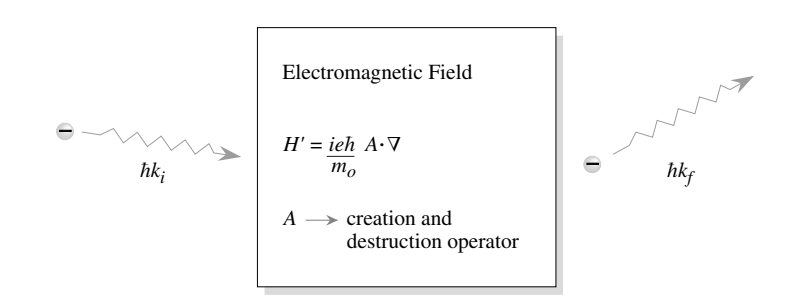
\includegraphics[width=\textwidth]{img/Scattering.png}
		\\[0.5em]
		\refstepcounter{figure}
		\textbf{Figure~\thefigure.} Schematic of the scattering process of an electron by the electromagnetic field.
		\label{fig:Scattering}
	\end{minipage}
\end{center}
The scattering process arises from this perturbation, where the electromagnetic field induces transitions in the electron states. In the second quantization framework, \( \mathbf{A} \) is quantized using photon creation and annihilation operators \( b^\dagger \) and \( b \), analogous to the harmonic oscillator treatment.\\
According to Fermi’s golden rule, the transition rate from an initial state \( |i\rangle \) to a final state \( |f\rangle \) is:
\begin{equation}
	W(i) = \frac{2\pi}{\hbar} \sum_f \left| \langle f | H' | i \rangle \right|^2 \delta \left( E_f - E_i \mp \hbar \omega \right)
\end{equation}
Here, the upper sign corresponds to photon absorption and the lower sign to emission.\\
The initial and final states are described by the electron's momentum and the photon number.

In the case of photon \textbf{absorption}, the states are:
\begin{align*}
	|i\rangle & = |k_i, n_{\text{ph}} \rangle     \\
	|f\rangle & = |k_f, n_{\text{ph}} - 1 \rangle
\end{align*}
\textbf{Emission:}
\begin{align*}
	|i\rangle & = |k_i, n_{\text{ph}}\rangle     \\
	|f\rangle & = |k_f, n_{\text{ph}} + 1\rangle
\end{align*}
Here, \(k_i\) and \(k_f\) denote the initial and final wavevectors of the electron, respectively, and \(n_{\text{ph}}\) is the initial photon occupation number. The vector potential \(A_0\) is defined as:
\begin{equation}
	A_0 = \sqrt{\frac{\hbar}{2 \omega \epsilon V}} \left(b^\dagger + b\right)
\end{equation}
In this expression, \(b^\dagger\) and \(b\) are the photon creation and annihilation operators. This form is chosen to be consistent with the magnitude \(|A_0|^2\) used previously.\\
When calculating matrix elements, we consider the photon operators separately. Let \( \mathbf{a} \) represent the polarization unit vector. Focusing on the matrix element due to the photon part only:
\textbf{Absorption:}
\begin{align*}
	\langle f | \mathbf{A} \cdot \nabla | i \rangle & \Rightarrow
	\sqrt{\frac{\hbar}{2 \omega \epsilon}} \left\langle k_f, n_{\text{ph}} - 1 \middle| \left(b^\dagger + b\right) \mathbf{a} \cdot \nabla \middle| k_i, n_{\text{ph}} \right\rangle             \\
	                                                & = \sqrt{\frac{\hbar}{2 \omega \epsilon}} \sqrt{n_{\text{ph}}} \left\langle k_f \middle| \mathbf{a} \cdot \nabla \middle| k_i \right\rangle
\end{align*}
\textbf{Emission:}
\begin{align*}
	\langle f | \mathbf{A} \cdot \nabla | i \rangle & \Rightarrow
	\sqrt{\frac{\hbar}{2 \omega \epsilon}} \left\langle k_f, n_{\text{ph}} + 1 \middle| \left(b^\dagger + b\right) \mathbf{a} \cdot \nabla \middle| k_i, n_{\text{ph}} \right\rangle                 \\
	                                                & = \sqrt{\frac{\hbar}{2 \omega \epsilon}} \sqrt{n_{\text{ph}} + 1} \left\langle k_f \middle| \mathbf{a} \cdot \nabla \middle| k_i \right\rangle
\end{align*}
It is crucial to notice the difference in prefactors: \( \sqrt{n_{\text{ph}}} \) appears for absorption, while \( \sqrt{n_{\text{ph}} + 1} \) appears for emission. This distinction will play a significant role in later discussions.
To proceed with calculating the rate for photon absorption—where a photon of energy \(\hbar \omega\) and momentum \(\hbar k_{\text{ph}}\) is absorbed by an electron—we will need to sum over all possible electron states which can allow such a process to occur.\\
\begin{center}
	\begin{minipage}{0.5\textwidth}
		\centering
		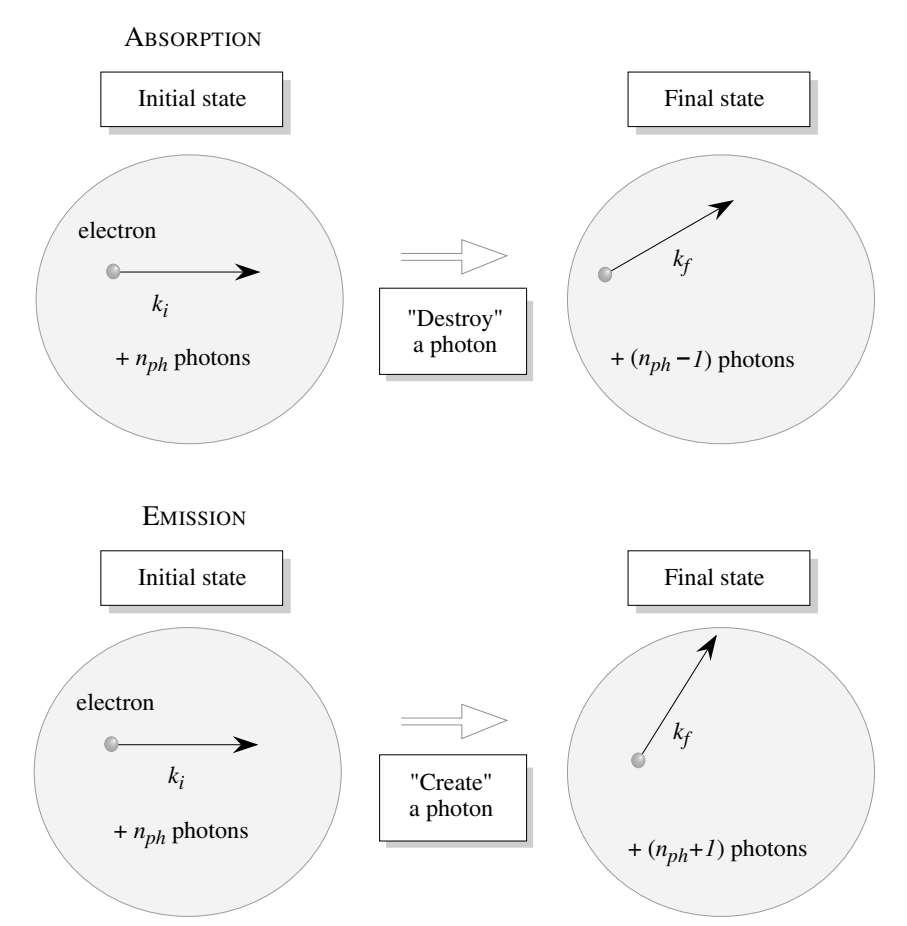
\includegraphics[width=\textwidth]{img/Abs&emiss.png}
		\\[0.5em]
		\refstepcounter{figure}
		\textbf{Figure~\thefigure.} (a) Schematic of a photon absorption process, where a photon is annihilated and the electron’s energy and momentum change.  
(b) Photon emission process, where a photon is generated as the electron transitions to a lower energy state. 
		\label{fig:Abs&emiss}
	\end{minipage}
\end{center}
The process of photon absorption involves the transfer of photon energy \(\hbar \omega\) to an electron. To compute the full scattering rate, we integrate over the final electron density of states:
\begin{equation}
W_{\text{abs}} = \frac{2\pi}{\hbar} \frac{e^2}{m_0^2} \left( \frac{\hbar n_{\text{ph}}}{2 \omega \epsilon} \right) \sum_{\text{final states}} \left| \int \psi_f^* (\mathbf{a} \cdot \mathbf{p}) e^{i \mathbf{k}_{\text{ph}} \cdot \mathbf{r}} \psi_i \, d^3r \right|^2 \delta(E_i - E_f + \hbar \omega)
\end{equation}
This expression includes a sum over all possible electronic final states for photon absorption, ensuring energy conservation. Alternatively, one might be interested in electron scattering from an initial state with momentum \(k_i\) to a final state with momentum \(k_f\), summing instead over photon states that enable this transition.\\
For photon emission, where an electron in state \(\hbar k_i\) emits a photon and transitions to \(\hbar k_f\), the corresponding rate is:
\begin{equation}
W_{\text{em}} = \frac{2\pi}{\hbar} \frac{e^2}{m_0^2} \left( \frac{\hbar(n_{\text{ph}} + 1)}{2 \omega \epsilon} \right) \sum_{\text{final states}} \left| \int \psi_f^* (\mathbf{a} \cdot \mathbf{p}) e^{-i \mathbf{k}_{\text{ph}} \cdot \mathbf{r}} \psi_i \, d^3r \right|^2 \delta(E_i - E_f - \hbar \omega)
\end{equation}
This emission rate can be broken into two components: one for stimulated emission and one for spontaneous emission:
\begin{equation}
W_{\text{em}} = W_{\text{st}} + W_{\text{spon}}
\end{equation}
where
\begin{equation}
W_{\text{st}} = \frac{2\pi}{\hbar} \frac{e^2}{m_0^2} \frac{\hbar n_{\text{ph}}}{2 \omega \epsilon} \sum_{\text{final states}} \left| \int \psi_f^* e^{-i \mathbf{k}_{\text{ph}} \cdot \mathbf{r}} (\mathbf{a} \cdot \mathbf{p}) \psi_i \, d^3r \right|^2 \delta(E_i - E_f - \hbar \omega)
\end{equation}
\begin{equation}
W_{\text{spon}} = \frac{2\pi}{\hbar} \frac{e^2}{m_0^2} \frac{\hbar}{2 \omega \epsilon} \sum_{\text{final states}} \left| \int \psi_f^* e^{-i \mathbf{k}_{\text{ph}} \cdot \mathbf{r}} \psi_i \, d^3r \right|^2 \delta(E_i - E_f - \hbar \omega)
\end{equation}
\textit{Stimulated emission} arises from the presence of photons already in the system, and the emitted photons are phase coherent with the initial ones. \textit{Spontaneous emission}, on the other hand, originates from quantum vacuum fluctuations (\(n_{\text{ph}} = 0\)) and results in photons that are phase-incoherent.\\
This distinction is fundamental in understanding the operational differences between devices such as LEDs and laser diodes.\\
When examining semiconductor states, we observe that the photon momentum \(\hbar k_{\text{ph}}\), for typical photon energies between 0.1 and 2.0 eV, is much smaller than the electron momentum. Therefore, momentum conservation requires that:
\begin{equation}
k_i = k_f
\end{equation}
In first-order perturbation theory, transitions triggered by photon absorption or emission are represented as "vertical" processes in the energy–momentum (\(E\)-\(k\)) diagram. This is particularly evident in interband transitions. When the photon momentum \(k_{\text{ph}}\) is small enough to be neglected, the approximation is referred to as the dipole approximation. Under this approximation, the momentum matrix element (the integral within the absolute value bars in the relevant transition rate equations) simplifies significantly. We denote this matrix element as \(p_{if}\).\\
Let us now consider the case where both the initial and final states follow the Bloch form. In the dipole approximation, the momentum matrix element becomes:
\begin{equation}
p_{if} = -i\hbar \int \psi^*_{\mathbf{k}_f \ell'} \, \nabla \psi_{\mathbf{k}_i \ell} \, d^3 r
\end{equation}
We define the initial and final Bloch states as follows:
\[
\begin{aligned}
    |i\rangle &= \psi_{\mathbf{k}_i, \ell} = e^{i \mathbf{k}_i \cdot \mathbf{r}} u_{\mathbf{k}_i \ell}, \\
    |f\rangle &= \psi_{\mathbf{k}_f, \ell'} = e^{i \mathbf{k}_f \cdot \mathbf{r}} u_{\mathbf{k}_f \ell'},
\end{aligned}
\]
where \( u_{\mathbf{k} \ell} \) denotes the cell-periodic part of the Bloch wavefunction, and \(\ell\), \(\ell'\) are band indices.\\
By applying the gradient operator to the initial state, the momentum matrix element simplifies into the following form:
\begin{equation}
p_{if} = \hbar \mathbf{k}_i \int \psi^*_{\mathbf{k}_f \ell'} \psi_{\mathbf{k}_i \ell} \, d^3 r 
- i\hbar \int u^*_{\mathbf{k}_f \ell'} \left( \nabla u_{\mathbf{k}_i \ell} \right) 
e^{i(\mathbf{k}_i - \mathbf{k}_f) \cdot \mathbf{r}} \, d^3 r
\end{equation}
\begin{figure}[H]
    \centering
    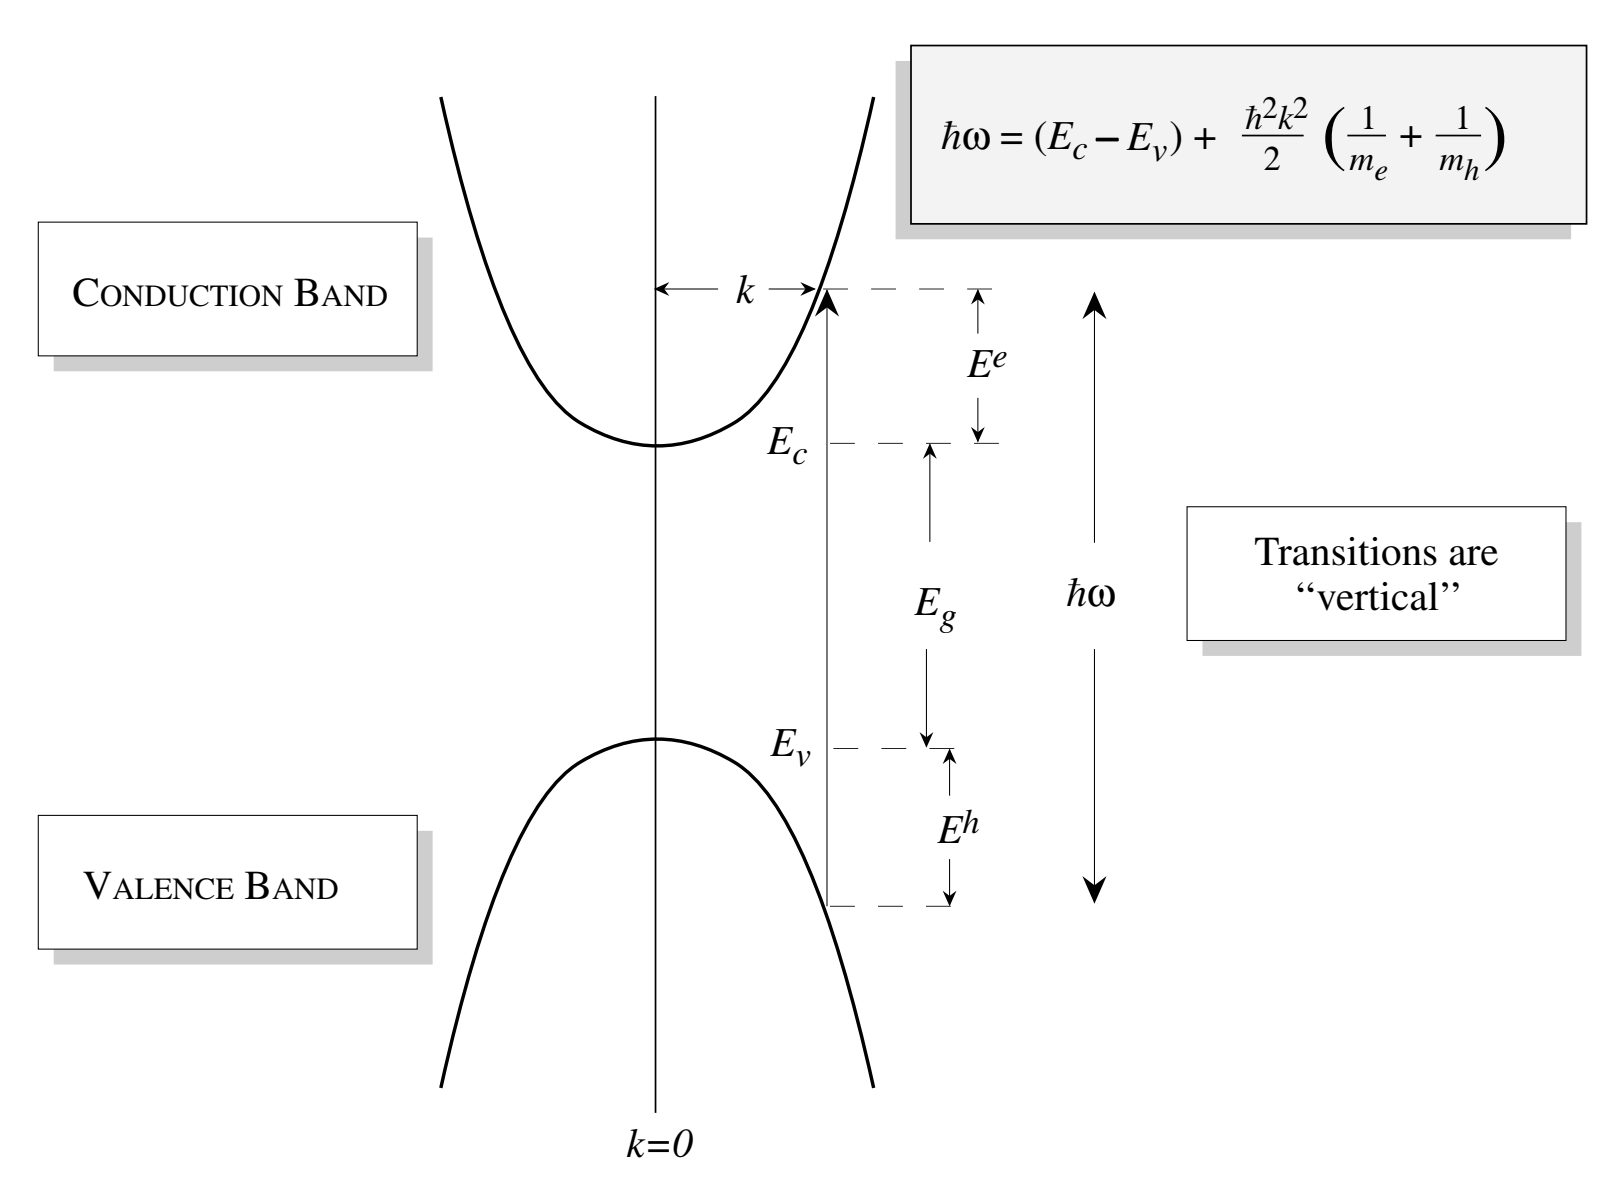
\includegraphics[width=0.8\textwidth]{img/transitions.png}
    \caption{Electron and hole energy levels at vertical \(\mathbf{k}\)-values. The transition energies are set by the photon energy and the effective masses of the carriers. Due to the negligible photon momentum, these transitions occur vertically in \(\mathbf{k}\)-space.
    }
    \label{fig:transitions}
\end{figure}



\section{Interband Transitions}

\subsection{Interband Transitions in Bulk Semiconductors}
\subsection{Interband Transitions in Quantum Wells}



\section{Indirect Interband Transitions}


\section{Intraband Transitions}
\subsection{Intraband Transitions in Bulk Semiconductors}
\subsection{Intraband Transitions in Quantum Wells}



\section{Charge Injection and Radiative Recombination}
\subsection{Spontaneous Emission Rate}
\subsection{Gain in a Semiconductor}



\section{Nonradiative Recombination}
\subsection{Charge Injection: Nonradiative Effects}
\subsection{Non-radiative Recombination: Auger Process}


\section{Semiconductor Light Emitters}
\subsection{Light Emitting Diode}
\subsection{Laser Diode}
\subsubsection{Optical Absorption, Loss and Gain}
\subsubsection{Laser Below and Above Threshold}